\documentclass[10pt]{article}
\usepackage[utf8]{inputenc}
\usepackage[T1]{fontenc}
\usepackage{lmodern}
\renewcommand{\familydefault}{\sfdefault}
\usepackage[letterpaper,margin=1.35cm,top=1.1cm,bottom=1.0cm]{geometry}
\usepackage{xcolor}
\usepackage{tikz}
\usetikzlibrary{calc,positioning}
\usepackage[most]{tcolorbox}
\usepackage{enumitem}
\usepackage{tabularx}
\usepackage{microtype}
\usepackage{amssymb}
\usepackage[hidelinks,
  pdftitle={CV - Juan Pablo Moreno Cadena},
  pdfauthor={Juan Pablo Moreno Cadena}]{hyperref}

% ====================================================================
% DIRECCION DEL SITIO: es lo unico que hay que cambiar.
% Sin "https://" y sin "/" al final. Ejemplo: mi-usuario.github.io/cv-unico
\newcommand{\sitio}{jpmcmoreno.github.io/cv-unico}
% ====================================================================

% TELEFONO: la version publica (la que se sube a GitHub) va sin telefono.
% Si existe el archivo telefono.tex junto a este (no se sube: esta en .gitignore),
% el CV lo incluye. Sirve para la version que envias directamente.
\IfFileExists{telefono.tex}{\input{telefono.tex}}{\newcommand{\telefono}{}}

\definecolor{ink}{HTML}{14213D}
\definecolor{soft}{HTML}{5C677D}
\definecolor{accent}{HTML}{E4572E}
\definecolor{accentdark}{HTML}{B93E1B}
\definecolor{paper}{HTML}{F6F4EF}
\definecolor{cA}{HTML}{2A9D8F}
\definecolor{cB}{HTML}{E9A23B}
\definecolor{cC}{HTML}{7B5EA7}

\pagestyle{empty}
\setlength{\parindent}{0pt}
\setlist[itemize]{leftmargin=1.1em,itemsep=1.2pt,topsep=2pt,parsep=0pt,label={\color{accent}\textbullet}}

% ---------- Boton "Dale un chance ;)" ----------
% #1 = ruta de la demo dentro del sitio, por ejemplo demos/chat/
\newcommand{\chance}[1]{%
  \href{https://\sitio/#1}{%
    \tcbox[on line,colback=accent,colframe=accentdark,boxrule=0.5pt,arc=6pt,
      left=5pt,right=5pt,top=1.6pt,bottom=1.6pt,boxsep=0pt,
      drop shadow={black!25,opacity=0.5}]{%
      \color{white}\bfseries\scriptsize Dale un chance ;)\;\(\blacktriangleright\)}%
  }%
}
\newcommand{\shorturl}[1]{\href{https://\sitio/#1}{\color{soft}\fontsize{6}{7}\selectfont\ttfamily \sitio/#1}}

\newcommand{\seccion}[1]{%
  \vspace{7pt}%
  {\color{ink}\bfseries\large #1}\\[-7pt]
  {\color{accent}\rule{2.2cm}{1.6pt}}{\color{ink!20}\rule{\dimexpr\linewidth-2.2cm}{0.4pt}}\par
  \vspace{4pt}%
}
\newcommand{\cargo}[3]{%
  {\color{ink}\bfseries #1}\hfill{\color{soft}\small #3}\\
  {\color{soft}\small #2}\par\vspace{1pt}%
}

% ---------- Tarjeta de demo ----------
% #1 titulo, #2 dibujo tikz, #3 descripcion, #4 respaldo, #5 ruta de la demo
\newcommand{\demo}[5]{%
  \begin{tcolorbox}[colback=paper,colframe=ink!18,boxrule=0.5pt,arc=5pt,
      left=6pt,right=6pt,top=5pt,bottom=5pt,height=3.55cm,valign=top]
    \begin{minipage}[t][2.95cm][t]{\linewidth}
      \begin{minipage}[c]{0.27\linewidth}\centering #2\end{minipage}\hfill
      \begin{minipage}[c]{0.70\linewidth}
        {\color{ink}\bfseries #1}\par\vspace{1.5pt}
        {\footnotesize #3}\par\vspace{1.5pt}
        {\color{soft}\scriptsize\itshape #4}
      \end{minipage}
      \vfill
      \chance{#5}\hfill\shorturl{#5}
    \end{minipage}
  \end{tcolorbox}%
}

\begin{document}

% ================= ENCABEZADO =================
\begin{tcolorbox}[enhanced,colback=ink,colframe=ink,arc=6pt,boxrule=0pt,
    left=12pt,right=12pt,top=9pt,bottom=9pt]
  \begin{minipage}[c]{0.60\linewidth}
    {\color{white}\bfseries\fontsize{21}{24}\selectfont Juan Pablo Moreno Cadena}\\[3pt]
    {\color{cB}\bfseries Desarrollador Python \textperiodcentered{} Datos e IA}\\[3pt]
    {\color{white!85!ink}\footnotesize Bogotá, Colombia \textperiodcentered{}
      \href{mailto:jpmcmoreno@gmail.com}{jpmcmoreno@gmail.com}\telefono}
  \end{minipage}\hfill
  \begin{minipage}[c]{0.36\linewidth}\raggedleft
    {\color{white}\footnotesize\itshape No me creas: pruébalo.}\\[2pt]
    {\color{white!80!ink}\scriptsize Cada botón naranja de este CV abre una\\
      demo en vivo de lo que digo que sé hacer.}
  \end{minipage}
\end{tcolorbox}

% ================= PERFIL =================
\seccion{Perfil}
{\small Matemático con experiencia construyendo automatizaciones en producción y modelos de
machine learning. Me gusta que el código se pueda \emph{usar}, no solo describir: por eso este CV
trae demos funcionando de cada habilidad.}

% ================= DEMOS =================
\seccion{Lo que sé hacer (y puedes probar)}
\begin{minipage}[t]{0.492\linewidth}
\demo{Servicios con IA generativa}{%
  
\begin{tikzpicture}[scale=0.8]
    \node[fill=ink!12,rounded corners=4pt,minimum width=1.25cm,minimum height=0.38cm,anchor=west] at (0,1.3) {};
    \node[fill=accent!75,rounded corners=4pt,minimum width=1.45cm,minimum height=0.38cm,anchor=east] at (2.2,0.72) {};
    \node[fill=ink!12,rounded corners=4pt,minimum width=1.0cm,minimum height=0.38cm,anchor=west] at (0,0.14) {};
  \end{tikzpicture}}
  {Chatbot propio consumiendo la API de un LLM. Conversación corta: es una demo.}
  {En Claro usé LLMs para clasificar respuestas abiertas de encuestas.}
  {demos/chat/}
\end{minipage}\hfill
\begin{minipage}[t]{0.492\linewidth}
\demo{Regresión lineal}{%
  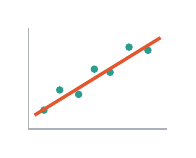
\begin{tikzpicture}[scale=0.8]
    \draw[ink!35,thin] (0,0)--(2.2,0) (0,0)--(0,1.6);
    \foreach \x/\y in {0.25/0.3,0.5/0.62,0.8/0.55,1.05/0.95,1.3/0.9,1.6/1.3,1.9/1.25}
      \fill[cA] (\x,\y) circle (1.7pt);
    \draw[accent,very thick] (0.1,0.22)--(2.1,1.45);
  \end{tikzpicture}}
  {Pon puntos con clics y mira cómo se ajusta la recta en tiempo real.}
  {En Claro predije la permanencia (en meses) de los empleados.}
  {demos/regresion/}
\end{minipage}

\vspace{1pt}
\begin{minipage}[t]{0.492\linewidth}
\demo{Clasificación}{%
  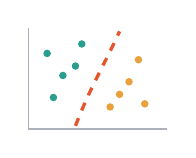
\begin{tikzpicture}[scale=0.8]
    \draw[ink!35,thin] (0,0)--(2.2,0) (0,0)--(0,1.6);
    \foreach \x/\y in {0.3/1.2,0.55/0.85,0.4/0.5,0.85/1.35,0.75/1.0}
      \fill[cA] (\x,\y) circle (1.7pt);
    \foreach \x/\y in {1.3/0.35,1.6/0.75,1.85/0.4,1.75/1.1,1.45/0.55}
      \fill[cB] (\x,\y) circle (1.7pt);
    \draw[accent,very thick,dashed] (0.75,0.05) .. controls (1.0,0.7) and (1.2,1.0) .. (1.45,1.55);
  \end{tikzpicture}}
  {Mueve los datos y observa cómo cambia la frontera de decisión.}
  {En Claro: modelo de fuga de empleados con 70\,\% de precisión.}
  {demos/clasificador/}
\end{minipage}\hfill
\begin{minipage}[t]{0.492\linewidth}
\demo{Clustering}{%
  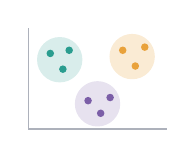
\begin{tikzpicture}[scale=0.8]
    \draw[ink!35,thin] (0,0)--(2.2,0) (0,0)--(0,1.6);
    \fill[cA!18] (0.5,1.1) circle (0.36); \fill[cB!22] (1.65,1.15) circle (0.36); \fill[cC!18] (1.1,0.4) circle (0.36);
    \foreach \x/\y in {0.35/1.2,0.55/0.95,0.65/1.25} \fill[cA] (\x,\y) circle (1.7pt);
    \foreach \x/\y in {1.5/1.25,1.7/1.0,1.85/1.3} \fill[cB] (\x,\y) circle (1.7pt);
    \foreach \x/\y in {0.95/0.45,1.15/0.25,1.3/0.5} \fill[cC] (\x,\y) circle (1.7pt);
  \end{tikzpicture}}
  {Elige el número de grupos y mira cómo se reagrupan los puntos.}
  {En Claro agrupé perfiles de liderazgo con métodos de clustering.}
  {demos/clusters/}
\end{minipage}

% ================= EXPERIENCIA =================
\seccion{Experiencia}
\cargo{Asistente de Datos Junior}{Risk Consulting Global Group \textperiodcentered{} Bogotá}{Ago 2025 -- Actualidad}
\begin{itemize}
  \item Construí una automatización en Python, desplegada en la plataforma interna, que recolecta y
        actualiza noticias con web scraping y consumo de una API externa.
        \chance{demos/scraping/}
\end{itemize}
\vspace{3pt}
\cargo{Docente Voluntario de Matemáticas}{Fundación Universitaria Konrad Lorenz \textperiodcentered{} Bogotá}{Feb 2025 -- May 2025}
\begin{itemize}
  \item Desarrollé herramientas didácticas interactivas en Python con Streamlit y material sobre
        geometría euclidiana, \LaTeX{} y teoría de números.
        \chance{demos/euclides/}
\end{itemize}
\vspace{3pt}
\cargo{Practicante de Analítica de Datos (People Analytics)}{Claro Colombia \textperiodcentered{} Bogotá}{Feb 2024 -- Jul 2024}
\begin{itemize}
  \item Modelos predictivos de fuga y de permanencia de empleados; clustering de perfiles de liderazgo.
  \item Optimicé los scripts de los modelos: de un mes a una semana de ejecución.
\end{itemize}
\vspace{3pt}
\cargo{Monitor de Lógica Matemática y de Fundamentos de Programación}{Fundación Universitaria Konrad Lorenz \textperiodcentered{} Bogotá}{2022}

% ================= EDUCACION + HABILIDADES =================
\begin{minipage}[t]{0.47\linewidth}
\seccion{Educación}
{\color{ink}\bfseries Matemáticas}\hfill{\color{soft}\small 2024}\\
{\color{soft}\small Fundación Universitaria Konrad Lorenz \textperiodcentered{} Mención de Honor}\\[3pt]
{\color{ink}\bfseries Ingeniería Industrial}\hfill{\color{soft}\small En curso}\\
{\color{soft}\small Corporación Universitaria Minuto de Dios}\\[3pt]
{\small Maratón Nacional de Programación 2021, 2022 y 2023}
\end{minipage}\hfill
\begin{minipage}[t]{0.49\linewidth}
\seccion{Habilidades}
{\small
\textbf{Lenguajes:} Python, SQL, Java\\[1.5pt]
\textbf{Datos y ML:} Pandas, NumPy, Scikit-learn\\[1.5pt]
\textbf{IA y automatización:} LLMs, APIs REST, web scraping\\[1.5pt]
\textbf{Herramientas:} Streamlit, Power BI, Git, \LaTeX}
\end{minipage}

\vfill
\begin{center}
{\color{soft}\scriptsize Todas las demos en un solo lugar:
\href{https://\sitio/}{\ttfamily \sitio}}
\end{center}

\end{document}
